\documentclass[..\EOYR.tex]{subfiles}

\begin{document}

\section{Barotropic Vorticity Diagnostics}
\label{SEC:Diagnostics}

Using the NEMO model, we are in the process of calculating barotropic vorticity diagnostics to further investigate the processes effecting the path of the Gulf Stream. These barotropic vorticity diagnostics have been used by \citep{Bell1999}, \citep{Gula2014} and \citep{Yeager2015} among others, to investigate the driving forces behind the vorticity budgets in the North Atlantic.\\

Two different diagnositcs will be calculated on each of the seven contributing terms to the momentum equations shown in equation (\ref{EQN:NEMOPrognostic}). The methods are similar to the approach taken in section (\ref{SSEC:EffectsOfTopography}) to find the JEBAR and bottom pressure torque terms and involve taking the curl of the vertically averaged and vertically integrated contributions.\\

Examining and comparing the results will help to highlight the leading terms driving the flow in different regions of the Gulf Stream. This may highlight key areas of bathymetry or emphasise the importance of the interaction with the DWBC.

\subsection{NEMO Ocean Model}
\label{SSEC:NEMO}

As the Barotropic Vorticity Diagnostics are being implemented in the NEMO model, it seems sensible to first introduce the model in a little more detail. \\
The Nucleus for European Modelling of the Ocean (NEMO) is a framework designed to allow for a flexible study of the ocean, it's dynamics and it's interaction with other climate systems \citep{Madec2011}. \\

The framework of NEMO allows the model to be configured in a variety of ways, choosing the resolution, numerical schemes and vertical coordinates according to your requirements. As discussed in section \ref{SEC:ModellingGulfStream}, the representation of the Gulf Stream can vary greatly depending on various aspects of the model chosen. The resolution can play a big role as discussed in \citep{Scaife2011a}, and \citep{Ezer2016b} showed that path of the Gulf Stream is sensitive also to the choice of vertical coordinates and bathymetrical representation. It is suitable then, for our requirements, as it will allow comparisons between a variety of different configurations in a way which can be problematic for most modellers (as noted in \citep{Ezer2016b}).\\

Within NEMO are many different engines designed to model different aspects of the ocean, these are OPA, which models the ocean dynamics and thermodynamics; LIM, which models the sea-ice dynamics and thermodynamics; and Top, modelling the biogeochemistry. For our purposes we are interested in OPA, which will we will run off the MONSooN super computer.\\
We can further narrow our interests for the current investigation within OPA down to the routines focusing on the ocean dynamics. This part of the model is located within the DYN directory of the code and is responsible for the momentum equations, which are key to the barotropic vorticity diagnostics and are the focus of this section. \\

The prognostic Prognostic Ocean dynamics equations used by NEMO (where $(NXT)$ stands for the next time step) are 
\begin{equation}
\begin{split}
    NXT = \underbrace{(VOR+KEG+ZAD)}_\text{Coriolis \& advection} + \underbrace{HPG+SPG}_\text{pressure gradient contributions} \\
    +\underbrace{LDF}_\text{lateral diffusion} +\underbrace{ZDF}_\text{vertical diffusion}.
\end{split}
\label{EQN:NEMOPrognostic}
\end{equation}


Here the Coriolis and advection terms are split into three parts: the vorticity $(VOR)$, the kinetic enery $(KEG)$ and the vertical advection $(ZAD)$.
In place of the Coriolis and advection terms shown here, in the flux formation, they can be replaced by a coriolis and advection term $(COR + ADV)$, however, for our purposes we wil be using the terms shown in equation (\ref{EQN:NEMOPrognostic}). The pressure gradient contributions consist of the hydrostatic pressure gradient $(HPG)$ and the surface pressure gradient $(SPG)$, and we also have the lateral $(LDF)$ and vertical diffusion $(ZDF)$ terms \citep{Madec2011}.
%\todo{Put citation elsewhere?}

Currently the diagnostics are being added to a $0.25\degree$ model using the z-coordinate bathymetry with partial setps (shown in Figure \ref{FIG:Coords} (b)).
Following the successful implementation of these diagnostics in one model formulation in NEMO, the intention is to then compare the results gained from running the calculations across different model resolutions and possibly different choices of vertical coordinates.

This could build on the review by \citep{Ezer2016b} by allowing for a more controlled comparison between models and allow an easier comparison and analysis of the results. Figure \ref{FIG:Ezer2016bFig8} (Fig. 8 from \citep{Ezer2016b}) shows the effect that the choice of model grid can have on the balance of the barotropic vorticity budget. With the various available configuration of NEMO, it will be interesting to further investigate this within a more controlled set up.

\begin{figure}[t]
    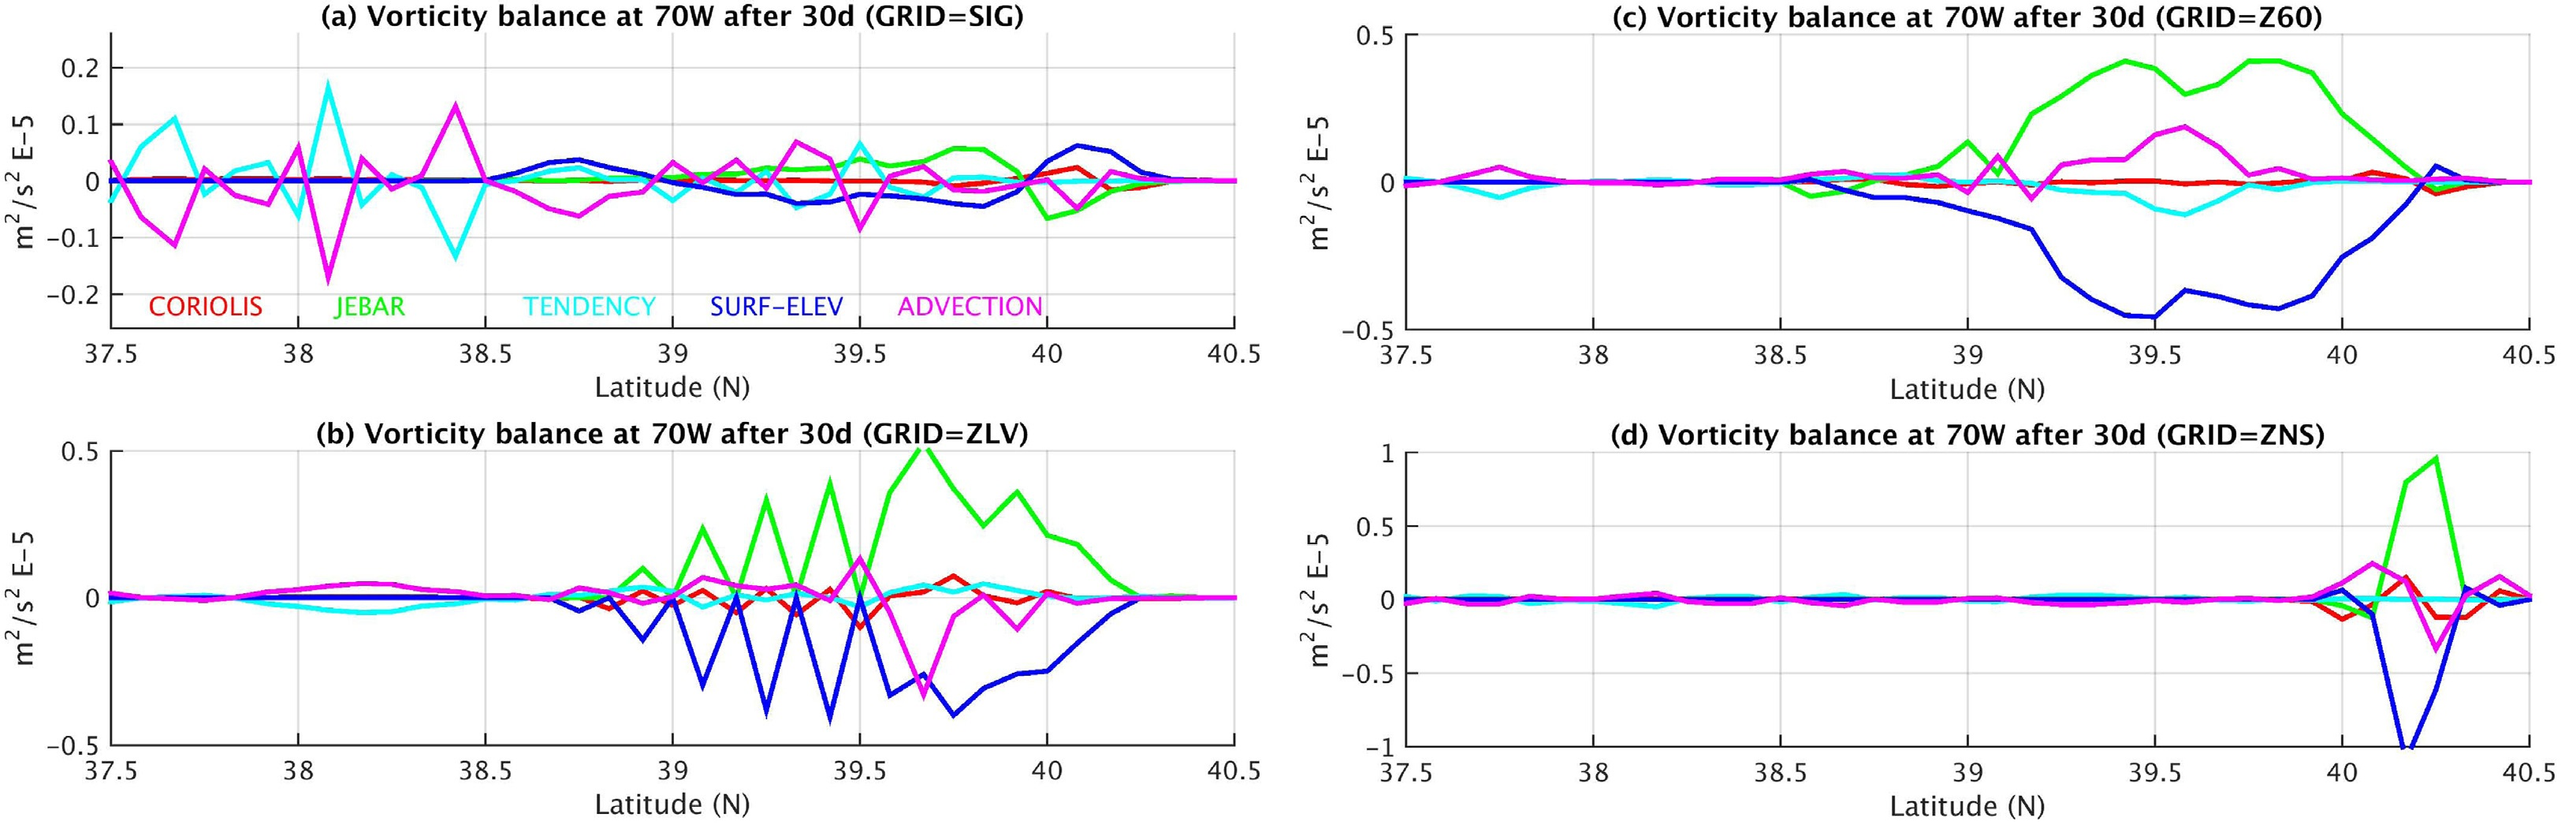
\includegraphics[width=\linewidth]{Figures/Ezer2016bFig8.jpg}
    \caption{Leading terms of the vorticity balance equation at 70$\degree$W after 30 days for experiments: (a) SIG (sigma coordinates), (b) ZLV (z-level coordinates with 21 layers), (c) Z60 (z-level coordinates with 61 layers) and (d) ZNS (z-level coordinates with no continental slope). Note the different scale in each panel. Each term has different color as indicated in (a). (Fig. 8 from \citep{Ezer2016b}) An example of the kind of results available from barotropic vorticity diagnostics.}
    \label{FIG:Ezer2016bFig8}
\end{figure}


\subsection{Barotropic Vorticity Diagnostics}
\label{SSEC:BVDiagnostics}


New code has been added to the NEMO model 
%\td{Pending validation?}
to calculate the two diagnostics. As each contribution to the momentum trend is calculated, it is passed to the subroutine which then calculates the required values.

The subroutine first calculates the vertical integral of the contribution, $\bar{u}$ and $\bar{v}$, over the height of the water column from the depth, $-H$, to the sea surface level $\eta$,
\begin{equation}
    \bar{u} = \int_{-h}^{\eta} u \,\text{d}z \,,\quad \bar{v} = \int_{-h}^{\eta} v \,\text{d}z 
    \label{UVBar}
\end {equation}


and then divide through by the height of the water column to obtain the vertical averages $\langle\bar{u}\rangle$ and $\langle\bar{v}\rangle$,
\begin{equation}
	\langle\bar{u}\rangle = \frac{1}{\eta + h}\int_{-h}^{\eta}u \,\text{d}z \,,\qquad \langle\bar{v}\rangle = \frac{1}{\eta + h}\int_{-h}^{\eta}v \,\text{d}z.
\label{UVBar}
\end{equation}


We now take the curl of each of these values to attain the two desired diagnostics
\begin{equation}
    \Omega = \frac{\partial \bar{v}}{\partial x} - \frac{\partial \bar{u}}{\partial y}
    \label{EQN:IntegratedDiagnostic}
\end{equation}


\begin{equation}
    \Omega_{avg} = \frac{\partial \langle\bar{v}\rangle}{\partial x} - \frac{\partial \langle\bar{u}\rangle}{\partial y}.
    \label{EQN:AveragedDiagnostic}
\end{equation}

    
Once the diagnostics have been calculated we can then compare the different contributions as in \citep{Yeager2015} and \citep{Gula2014}. Using equation (\ref{EQN:Streamfunction}) we can also calculate the barotropic streamfunction driving the flow.\\



\end{document}
